\section{Procesamiento Paralelo}
\label{sec:procesamiento_paralelo}
%Pequeña introduccion de que es el procesamiento paralelo
% - Explicar que existen tres caminos de paralelizacion, aunque la tercera
%   la que está basada en redes de neuronas, es un sistema que difiere al que
%   se viene viendo.

Diversos autores\cite{moldovan93, trobec2018} describen en profundidad diferentes modelos que
extienden a la arquitectura tradicional de Von Neumann para lograr
paralelización\footnote{No es el objetivo de este documento dar una descripción minuciosa de los
diferentes modelos teóricos de paralelización.}. Esta se logra mediante la separación de una tarea $T$, en subtareas
$T_{1}, T_{2}, \ldots , T_{n}$ (Diferentes autores adoptan este concepto con el
término de \textit{\gls{pipelining}}~\cite{hyde98, trobec2018}). Luego para lograr el cometido, 
más de una de las $T_{n}$ tareas debe realizarse al mismo tiempo, sin malinterpretar la
realización de una tarea de manera muy velóz con realizarla al mismo tiempo que
otras~\cite{hyde98}.

Las diferentes soluciones para procesamiento paralelo se desenvolvieron hasta
llegar a presentar uno de los siguientes tres tipos de
paralelismo\cite{trobec2018}:

\begin{itemize}
\item Los {\bf Sistemas de Memoria Compartida} que se componen de múltiples unidades de procesamiento
unidas a una memoria.
\item Los {\bf Sistemas Distribuidos} que se componen de equipos con sus propias unidades de procesamiento
y memoria, comunicados a traves de una conexión de red de alta velocidad. Este
es el caso que nos compete en este documento y es tratado en la Sección
\ref{sec:procesamiento_distribuido}.
\item Las {\bf Unidades de Procesamiento Gráfico} utilizadas como co-procesadores por su
capacidad de paralelizar grandes cantidades de operaciones.
\end{itemize}

Diferentes enfoques existen a la hora de aplicar el \gls{pipelining} mencionado
anteriormente, y estos no son recientes sino que datan desde la década de 1990.
Con el pasar del tiempo se fueron creando más enfoques y especializando los
casos generales que se tenían en un principio. Ejemplo de algunas
especializaciones son los enfoques que se ven en la cátedra de Paradigmas y Lenguajes 
de Programación\cite{pylp1}, en donde se denomina a este problema
\textit{Descomposicion}, y de ahí surgen las diferentes especializaciones:
Dominio, Funcion, Recursiva, Mixta.

Para este documento solamente se tienen en cuenta dos de las tres que se 
proponen por Fountain~\cite{fountain1994}: Paralelización de Datos y
Paralelización de Funciones.

La paralelización de datos y la paralelización de funciones puede encontrarse 
en diferentes niveles de la arquitectura
del computador, algunos ejemplos van desde, el procesador como lo describe
Hyde~\cite{fountain1994}, pasando por el compilador~\cite{clark1997}, llegando
a la aplicación~\cite{wolters1995}, etc. Este 
documento cubre únicamente a casos que son aplicados a nivel de aplicación.

\subsection{Paralelización de Datos}
\label{ssec:paralelizacion_de_datos}

\begin{tcolorbox}
La idea principal detrás de este enfoque a la hora de aplicar el {\it pipelining}
consiste en que un programa secuencial puede ser transformado a un
programa paralelo, realizando ejecuciones de copias idénticas de dicho programa como
tareas separadas, a las cuales se les brinda simplemente parte de los datos
iniciales~\cite{haveraaen2000}.
\end{tcolorbox}

En la figura \ref{fig:sin_paralelizacion_datos} se presenta una aplicación que
está corriendo sobre un núcleo aleatorio en un ordenador. En este ejemplo no se tiene
presente la paralelización, $D$ representa los datos sobre los cuales está
trabajando la \textit{Aplicación}.

\begin{figure}[h]
  \centering
  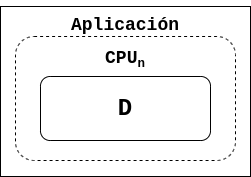
\includegraphics[width=0.3\linewidth]{figuras/procesamiento_paralelo_sin_paralelizacion_datos.png}
  \caption{Aplicación sin paralelización}
  \label{fig:sin_paralelizacion_datos}
\end{figure}

En la figura \ref{fig:con_paralelizacion_datos} se presenta la misma
aplicación (esta vez se la denomina \textit{app}). En este ejemplo
los datos representados por $D$ anteriomente, se
dividien en $D_{n}$ secciones más pequeñas que son distribuidas a distintos
núcleos de procesamiento \footnote{en el ejemplo se utilizan 4, aunque pueden ser más
núcleos dentro de un procesador}. Una copia idéntica de la aplicación (Figura
\ref{fig:sin_paralelizacion_datos}) se encuentra corriendo en cada uno de los
cuatro núcleos del ordenador, cada una de estas copias idénticas se
encuentra trabajando con datos distintos (ya que a cada una de las copias le
toca una sección $D_{n}$ diferente).

\begin{figure}[h]
  \centering
  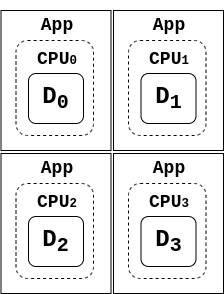
\includegraphics[width=0.3\linewidth]{figuras/procesamiento_paralelo_con_paralelizacion_datos.png}
  \caption{Aplicación con paralelización de datos}
  \label{fig:con_paralelizacion_datos}
\end{figure}

Una interpretación alternativa se puede ver en la figura
\ref{fig:con_paralelizacion_datos_alt}, este gráfíco se puede leer como ``Una
aplicación que se encuentra corriendo sobre distintos nucleos, con distintos
fragmentos de los datos originales''

\begin{figure}[h]
  \centering
  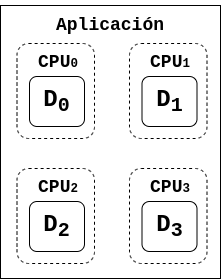
\includegraphics[width=0.3\linewidth]{figuras/procesamiento_paralelo_con_paralelizacion_datos_alt.png}
  \caption{Aplicación con paralelización de datos - Representación alternativa}
  \label{fig:con_paralelizacion_datos_alt}
\end{figure}


En la bibliografía existen implementaciones en diferentes sub áreas de las Ciencias de la
Computación con este enfoque presente, el procesamiento de
imágenes~\cite{pang2009}, el manejo de bases de
datos~\cite{zakharov2019} y la inteligencia artificial~\cite{hajj2015} por
nombrar algunos ejemplos. 

Para un ejemplo simple y concreto se propone lo siguiente: 

\begin{tcolorbox} \label{ej:1} 
  Se presenta la tarea de encontrar el valor mínimo dentro de un arreglo 
  $A = [a_{0}, a_{1}, \ldots , a_{n-2}, a_{n-1}]$.
\end{tcolorbox}

Se puede proceder sin aplicar paralelización de datos, y realizar una
aplicación que recorra los $n$ elementos del arreglo, realice las
comparaciones necesarias y devuelva el valor mínimo, o se puede
optar por la opción con paralelización de datos, una solución con este enfoque 
será fraccionar el arreglo con $A$ en, por ejemplo, 2 partes $A_{1}$ y
$A_{2}$. Luego se procede a distribuir estas dos partes $A_{1}$ y
$A_{2}$ a diferentes instancias de la aplicación que calcula el mínimo, 
de esta manera se tendrán dos núcleos de procesamiento que trabajarán en un
problema de menor tamaño (ya que
cada uno va a trabajar únicamente con el 50\% de los datos), y al final
solamente hará falta realizar una comparación entre los mínimos que
encuentren las dos instancias de la aplicación.

Cabe destacar que algunos problemas pueden surgir a la hora de particionar
datos si esto se hace sin nignun análisis, un ejemplo de esto puede ser
considerado en el escenario en donde ocurre
la división de una imagen en partes más pequeñas para su análisis en forma
paralela~\cite{oshitani1999}. También se hace presente la limitación que impone
la ley de Amdhal\footnote{``El incremento máximo de velocidad (la cantidad máxima de
procesadores que pueden ser utilizados de manera efectiva) es la inversa de la
fracción de tiempo que la tarea toma para finalizar en un solo
hilo'' \cite{rodgers1985}}.
% \begin{figure}[h]
  \centering
  \label{fig:paralelizacion_datos}
  \resizebox{!}{5cm}{%
    \begin{tikzpicture}
      % Dato
      \draw (0,4.75) rectangle (5,8.75) node[midway,blue]{\texttt{Datos}: $1,2,3,4,5,6,7,8,9,10$};

      % Datos
      \draw (9, 10) rectangle(10.5,11.5) node[midway,blue]{$1,2$};
      \draw (9, 8) rectangle (10.5,9.5) node[midway,blue]{$3,4$};
      \draw (9, 6) rectangle (10.5,7.5) node[midway,blue]{$5,6$};
      \draw (9, 4) rectangle (10.5,5.5) node[midway,blue]{$7, 8$};
      \draw (9, 2) rectangle (10.5,3.5) node[midway,blue]{$9, 10$};
    \end{tikzpicture}
  }
  \caption{Concepto paralelización de datos}
\end{figure}


\subsection{Paralelización de Funciones}
\label{ssec:paralelizacion_de_funciones}

\begin{tcolorbox}
  Este enfoque a la paralelización toma otro camino a la hora de aplicar el
  \textit{pipelining}, este acercamiento
  no fracciona los datos sino que transforma la tarea a un gráfo de 
  dependencias en donde cada nodo corresponde a una operación a ser realizada
  para cumplir la tarea. Y lo que trata de hacer es ejecutar la mayor
  cantidad de tareas al mismo tiempo~\cites{meng2013, liu2019, zhou2020,
  lin2021}.
\end{tcolorbox}

Esta idea de distribuir los datos a diferentes unidades funcionales que se
encarguen de realizar una tarea sobre los datos mencionados se presenta en la
figura \ref{fig:con_paralelizacion_funciones}.

% En la figura \ref{fig:con_paralelizacion_datos} se presenta la misma
% aplicación (esta vez se la denomina \textit{app}). En este ejemplo
% los datos representados por $D$ anteriomente, se
% dividien en $D_{n}$ secciones más pequeñas que son distribuidas a distintos
% núcleos de procesamiento \footnote{en el ejemplo se utilizan 4, aunque pueden ser más
% núcleos dentro de un procesador}. Una copia idéntica de la aplicación (Figura
% \ref{fig:sin_paralelizacion_datos}) se encuentra corriendo en cada uno de los
% cuatro núcleos del ordenador, cada una de estas copias idénticas se
% encuentra trabajando con datos distintos (ya que a cada una de las copias le
% toca una sección $D_{n}$ diferente).

Aquí se puede observar que lo que se subdivide no son los datos, sino que lo que
se está subdividiendo es la funcionalidad que compone a la tarea $T$, aquí cada
$o_{n}$ es una operación claramente delimitada dentro de la aplicación, y $D$
representa a los datos con los que se va a trabajar.

\begin{figure}[h]
  \centering
  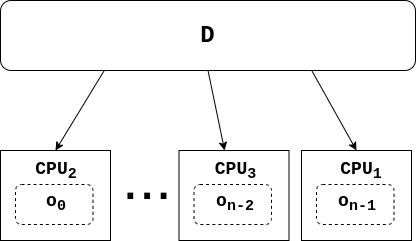
\includegraphics[width=0.65\linewidth]{figuras/procesamiento_paralelo_con_paralelizacion_func.png}
  \caption{Aplicación con paralelización de funciones}
  \label{fig:con_paralelizacion_funciones}
\end{figure}


Un ejemplo concreto para este enfoque se presenta a continuación:

\begin{tcolorbox}
  Dada una imagen, se presenta la tarea de determinar si en dicha imagen se
  encuentra presente algún rostro, vehículo, gato o planta.
\end{tcolorbox}

Por lo que se puede decir que la tarea $T$ se compone de la siguiente manera

\begin{equation} \label{eq-tareas-nodos}%
  T = [o_{0}, o_{1}, o_{2}, o_{3}]
\end{equation}

En donde se tiene que,

\begin{tabular}{l   l}
$o_{0}$ & Buscar rostro \\
$o_{1}$ & Buscar vehículo \\
$o_{2}$ & Buscar planta \\
$o_{3}$ & Buscar gato\\
\end{tabular}

\vspace{1cm}

Cada $o_{n}$ en la ecuación \ref{eq-tareas-nodos} representa un nodo del gráfo 
mencionado anteriormente. Ahora toca analizar y determinar
cuales de las $o_{n}$ operaciones se pueden realizar al mismo tiempo.

Una cuestion esencial en este ejemplo es identificar el hecho de que ninguna
operación $o_{n}$ depende de alguna operación.
% $o_{m}$ $\forall m, n \in
% \mathbb{N}| 0 \leq m, n \leq 3$
Esto es visible a la hora de realizar diversas preguntas con
respecto al contexto, 
\begin{itemize}
    \item ¿Es necesario determinar si existe o no un rostro para poder iniciar
      el análisis y determinar si la imagen contiene un vehiculo, gato o
      planta? No, entonces, {\it Buscar rostro} es independiente a las demás
      operaciones.
    \item ¿Es necesario determinar si existe un vehiculo en la imagen para
      poder iniciar el análisis y determinar si la imagen contiene un rostro,
      gato o planta? No, entonces, {\it Buscar vehículo} es independiente a las
      demás operaciones.
\end{itemize}

El análisis anterior debe continuar hasta que se analicen las $o_{n}$
operaciones. Habrán veces en donde dos o más operaciones no podrán ser ejecutadas de
manera paralela, esto puede darse porque una (también pueden ser varias) de ellas 
depende de los resultados que se obtengan de otra u otras operaciones.

En el caso del ejemplo para la sección, esta apreciación y el análisis que se
realizó permite definir que todas las operaciones que componen a la tarea $T$
se pueden ejecutar de manera paralela por el mismo dato.
